\id{IRSTI 65.65.03}{}

\begin{articleheader}
\sectionwithauthors{A. Dalabayev}{DETERMINATION OF TRANSISOMERS OF FATTY ACIDS IN BAKERY AND CONFECTIONERY PRODUCTS}

{\bfseries
A. Dalabayev\alink{https://orcid.org/0000-0001-7811-0697}
}
\end{articleheader}

\begin{affiliation}
Astana branch «Kazakh research institute of processing and food
industry» LTD, Astana, Kazakhstan

\raggedright \textsuperscript{\envelope }Corresponding-author: dalabaev\_askhat@mail.ru
\end{affiliation}

Currently, the problem of high content of trans-isomers of fatty acids
in food products has become widely discussed throughout the world, as
large-scale studies have proven the connection between the consumption
of trans fats and the development of cardiovascular diseases, type II
diabetes, and obesity. In 2018, the upper limit of trans-isomers of
fatty acids was regulated in TR CU 024/2011 «Technical regulations for
oil and fat products» no more than 2\% of the fat content in the
product. However, these restrictions apply exclusively to oil and fat
products, and for other types of food products there are no such
restrictions and the content of TFA in them is not regulated. In this
regard, the purpose of the research is to assess the food safety of
bakery and confectionery products obtained using margarines based on
hydrogenated oils produced from domestic raw materials of the Republic
of Kazakhstan. The article presents the incidence of circulatory system
diseases and changes in prices for margarine products. The content of
trans-isomers of fatty acids in 10 types of bakery and confectionery
products was determined. It was found that the content of trans-isomers
in all the studied samples does not exceed 2\%, and the daily intake
rate of trans-isomers of fatty acids was also determined.

{\bfseries Keywords:} transisomers of fatty acids, hydrogenated oils,
margarine, vegetable fat, bakery products, confectionery products, IR
spectroscopy.

\begin{articleheader}
{\bfseries НАН ЖӘНЕ КОНДИТЕРЛІК ӨНІМДЕРДІҢ ҚҰРАМЫНДАҒЫ МАЙ ҚЫШҚЫЛДАРЫ ТРАНСИЗОМЕРЛЕРІНІҢ МӨЛШЕРІН АНЫҚТАУ}

{\bfseries А.Б. Далабаев}
\end{articleheader}

\begin{affiliation}
Астана филиалы ЖШС Қазақ қайта өңдеу және тағам
өнеркәсіптері ғылыми-зерттеу институты, Астана, Қазақстан,

е-mail: dalabaev\_askhat@mail.ru
\end{affiliation}

Қазіргі уақытта азық-түлік өнімдеріндегі май қышқылдары
трансизомерлерінің жоғары деңгейі мәселесі бүкіл әлемде кеңінен
талқылануда, өйткені ауқымды зерттеулер транс майларын тұтыну мен
жүрек-қан тамырлары ауруларының, II типті қант диабетінің және
семіздіктің дамуы арасындағы байланысты дәлелдеді.2018 жылы май
қышқылдарының трансизомерлерінің жоғарғы шегі КО ТР 024/2011 «Май және
тоң-май өнімдерінің техникалық регламентінде өнімдегі май мөлшерінің
2\%-дан аспауы керектігін орнатты. Дегенмен, бұл шектеулер тек май және
май өнімдеріне қатысты, ал тамақ өнімдерінің басқа түрлері үшін мұндай
шектеулер жоқ және олардағы трансизомерлерінің мөлшері реттелмейді.
Осыған байланысты зерттеудің мақсаты Қазақстан Республикасының отандық
шикізатынан өндірілген гидрогенизацияланған майлар негізіндегі
маргариндерді қолдану арқылы алынған нан және кондитерлік өнімдердің
тағамдық қауіпсіздігін бағалау болып табылады. Мақалада қан айналымы
жүйесі ауруларының жиілігі мен маргарин өнімдерінің бағасының өзгеруі
тамамдалған. Нан және кондитерлік өнімдердің 10 түріндегі май
қышқылдарының трансизомерлерінің мөлшері анықталды. Барлық зерттелген
үлгілердегі трансизомерлердің мөлшері 2\%-дан аспайтыны анықталды,
сонымен қатар май қышқылдарының транс-изомерлерінің тәуліктік қабылдау
нормасы да анықталды.

{\bfseries Түйін сөздер:} май қышқылдарының трансизомерлері,
гидрогенизацияланған майлар, маргарин, өсімдік майы, нан өнімдері,
кондитерлік өнімдер, ИҚ спектроскопиясы.
\newpage
\begin{articleheader}
{\bfseries ОПРЕДЕЛЕНИЕ СОДЕРЖАНИЯ ТРАНСИЗОМЕРОВ ЖИРНЫХ КИСЛОТ В
ХЛЕБОБУЛОЧНЫХ И КОНДИТЕРСКИХ ИЗДЕЛИЯХ}

{\bfseries А.Б. Далабаев}
\end{articleheader}

\begin{affiliation}
Астанинский филиал ТОО «Казахский
научно-исследовательский институт перерабатывающей и пищевой
промышленности», Астана, Казахстан,

е-mail: dalabaev\_askhat@mail.ru
\end{affiliation}

В настоящее время проблема высокого содержания трансизомеров жирных
кислот в пищевых продуктах стала широко обсуждаемой во всём мире, так
как в проведённых крупномасштабных исследованиях была доказана связь
потребления трансжиров с развитием заболеваний сердечно-сосудистой
системы, сахарного диабета II типа, ожирения. В 2018 году произошла
регламентация верхнего предельного уровня трансизомеров жирных кислот в
ТР ТС 024/2011 «Технический регламент на масложировую продукцию» не
более 2\% от содержания жира в продукте. Однако, эти ограничения
касаются исключительно для масложировых продуктов, а для остальных видов
пищевых продуктов отсутствуют данного рода ограничения и содержание ТЖК
в них не регулируются. В связи с этим, целью исследований является
оценка пищевой безопасности хлебобулочных и кондитерских изделий
полученных с использованием маргаринов на основе гидрогенизированных
масел произведенных из отечественного сырья РК. В статье приведены по
заболеваемости системы кровообращения и изменение цен на маргариновую
продукцию. Определены содержание трансизомеров жирных кислот в 10 видах
хлебобулочных и кондитерских изделий. Установлено, что содержание
трансизомеров во всех исследуемых образцах не превышает 2\%, также
опеделена суточная норма потребления трансизомеров жирных кислот.

{\bfseries Ключевые слова:} трансизомеры жирных кислот, гидрогенизированные
масла, маргарин, растительный жир, хлебобулочные изделия, кондитерские
изделия, ИК спектроскопия.

\begin{multicols}{2}
{\bfseries Introduction.} One of the recipe components of bakery and
confectionery products are fats. Their content in the recipe can vary
widely from 5\% and higher {[}1-3{]}. Both vegetable oils (sunflower,
rapeseed, cottonseed, corn) and margarines or special-purpose fats are
used as fat components {[}4{]}. Despite the restriction in the countries
of the Customs Union, including our country, since 2018 of trans-isomers
of fatty acids (TFA) in oil and fat products, as has been written in the
media in recent years, their amount in hard margarines and
special-purpose fats for the bakery and confectionery industry remains
high - up to 20\% of the fat content in the product according to TR CU
024/2011 «Technical Regulations for Oil and Fat Products». In bakery and
confectionery products using hydrogenated fats, the amount of TFA can
reach up to 6.7\%, and in potato chips - up to 35\% {[}5-8{]}. As a
result, with the consumption of 100 g of baked goods or flour
confectionery, the human body can receive 5 times more TFA than the WHO
recommended norms - 1\% of the daily caloric intake, but is this really
the case in the realities of the Republic of Kazakhstan?

The danger of TFA is associated, first of all, with an almost 2-fold
increase in the risk of cardiovascular diseases due to an increase in
cholesterol and low-density lipoprotein levels. As a result, the risk of
sudden death increases {[}9,10{]}. The impact of TFA consumption on
public health is actively studied in foreign countries; in our country,
studies of this kind have not been conducted. The changes that occurred
with the tightening of technical regulations in 2018 also require an
assessment of the changing situation. The prevalence of
alimentary-dependent diseases does not tend to decrease, which also
determines the relevance of this study. At the same time, the impact of
restrictions on TFA to 2\% in 2018 for the Republic of Kazakhstan was
studied.8 years have passed since the introduction of this restriction;
during this period, the dynamics of population mortality from diseases
of the circulatory system was studied, since most studies in recent
years indicate a negative impact of TFA on the circulatory system.
According to the ASPR RK Bureau of National Statistics, the average
mortality rate for diseases of the circulatory system before the
introduction of restrictions was 0.2\%, and after 0.18\%, while on
average over the past 6 years the mortality rate has decreased by only
0.02\%, which does not give a more tangible effect for the population of
the Republic of Kazakhstan. If we calculate the average number of
deaths, then the introduction of restrictions led to a reduction in
deaths by an average of 6 people over 6 years. Interestingly, the
indication of the TFA content on food labels saved up to 500 lives per
year in the United States due to a decrease in the incidence of
cardiovascular diseases {[}11{]}. We also analyzed the change in retail
prices for margarine before and after the introduction of restrictions,
the results are presented in Figure 1.
\end{multicols}

\begin{figure}[H]
	\centering
	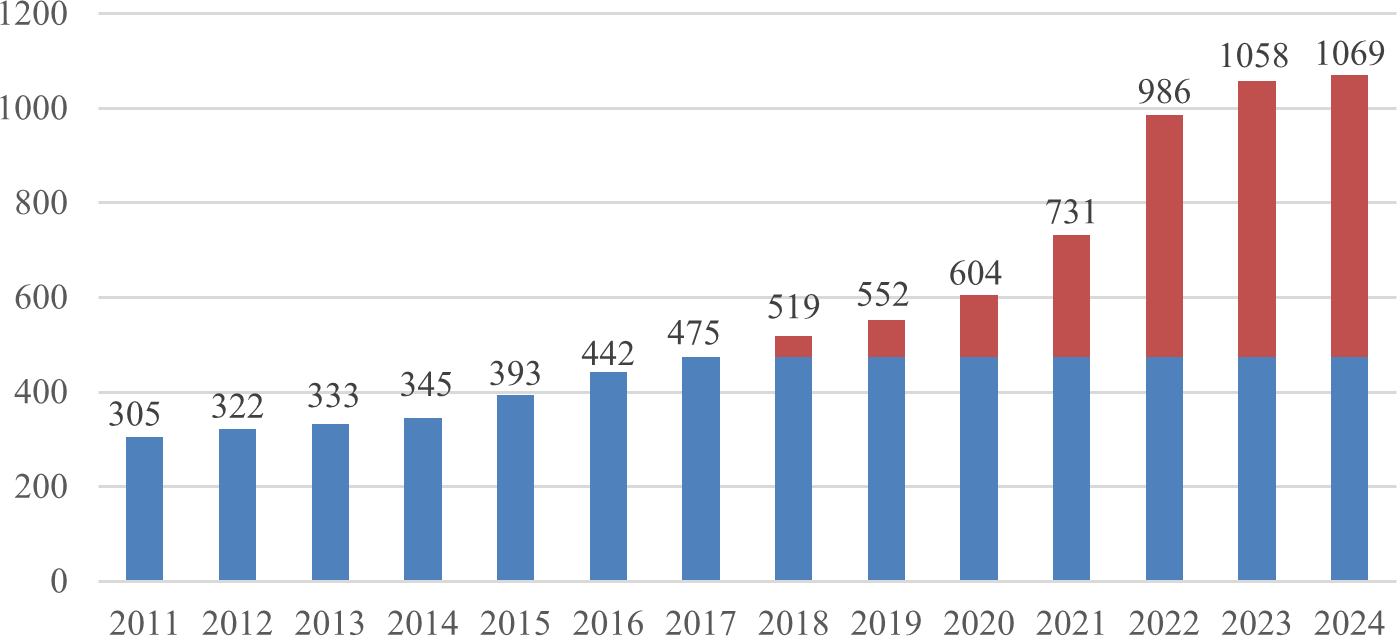
\includegraphics[width=0.8\textwidth]{media/pish4/image4}
	\caption*{Fig.1 - Change in retail prices for margarine for 2011-2024}
\end{figure}

\begin{multicols}{2}
As can be seen from Figure 1, retail prices for margarines have grown
rapidly after the introduction, if we take into account the average
price values, then for 2018-2024 they have grown almost 2,1 times
compared to 2011-2017. The introduction of restrictions on TFA to 2\% of
the fat content for oil and fat products led to an increase in the
import of palm oil, an increase in the cost of margarines by 2,1 times,
and did not give a significant effect in improving the health of the
population of the Republic of Kazakhstan. In this regard, the purpose of
the research is to assess the food safety of bakery and confectionery
products obtained using margarines based on hydrogenated oils produced
from domestic raw materials of the Republic of Kazakhstan.

{\bfseries Materials and methods.} The objects of the study are:
hydrogenated oil, margarine, sugar cookies, oatmeal cookies, crackers,
gingerbread, prolong cookies, waffles, flatbreads, buns, fudge,
confectionery glaze. The studies were conducted from September 2024 to
January 2025.

For the studies, vegetable fat of 99.7\% fat content, based on
hydrogenated oils from Maslo-Del LLC, with a transisomer content of
10\%, was provided; margarine «3 wishes» Pampushka, 55\% fat content of
Eurasian Foods JSC, was purchased as a control sample. Experimental
baking was carried out in the laboratories of processing oilseed raw
materials and deep processing of plant products, using a U1-ETK dough
mixer, SB 500-70 dough sheeter, XL 413 proofer and HV 693 convection
oven.

After the experimental baking, the mass fraction of fat in the finished
bakery and confectionery products was determined according to GOST
5668-2022 and GOST 31902-2012. The analyzed sample of products was
weighed on scales with the result recorded in grams to the third decimal
place, placed in a filter paper cartridge. The cartridge with the sample
was placed in a Soxhlet apparatus and fat was extracted with diethyl
ether for 5 hours. The resulting mixture was evaporated in a water bath
in a fume hood. The flask with the obtained fat was dried in a drying
cabinet at a temperature of 100°C until constant weight, then cooled in
a desiccator for 20 min. In this way, 100 g samples of extracted fat
were prepared for each product.

The content of trans isomers in the extracted fats was determined
according to GOST 33441-2015 «Vegetable oils. Determination of quality
and safety indicators by near infrared spectroscopy» on an IR Fourier
spectrometer IR Spirit-TX (Shimadzu, Japan). Absorption spectra were
recorded in the range of 4000-400 cm\textsuperscript{-1}, with a
resolution of 8 cm\textsuperscript{-1}, 64 scans, with subsequent
mathematical calculation of the values of the determined indicators.

Mass fraction of trans isomers of unsaturated fatty acids in products X,
\%, according to GOST R 54687 - 2011 «Confectionery products. The method
for determining the mass fraction of trans-isomers of unsaturated fatty
acids» is calculated using the formula:

\begin{equation}
X = \frac{Y \times T}{100}
\end{equation}

where, \emph{Y} - mass fraction of fat in the product under study, \%;

\emph{Т} - mass fraction of trans fatty acids, \%.

Statistical analyses were performed using the Statgraphics Centurion 19
software package.

{\bfseries Results and discussion.} Experimental baking of bakery and
confectionery products was carried out at the Astana branch of the
Kazakh Research Institute of Processing and Food Industry LLP. The
results of the experimental and control baking are presented in Figure
2. 
\end{multicols}

\begin{figure}[H]
	\centering
	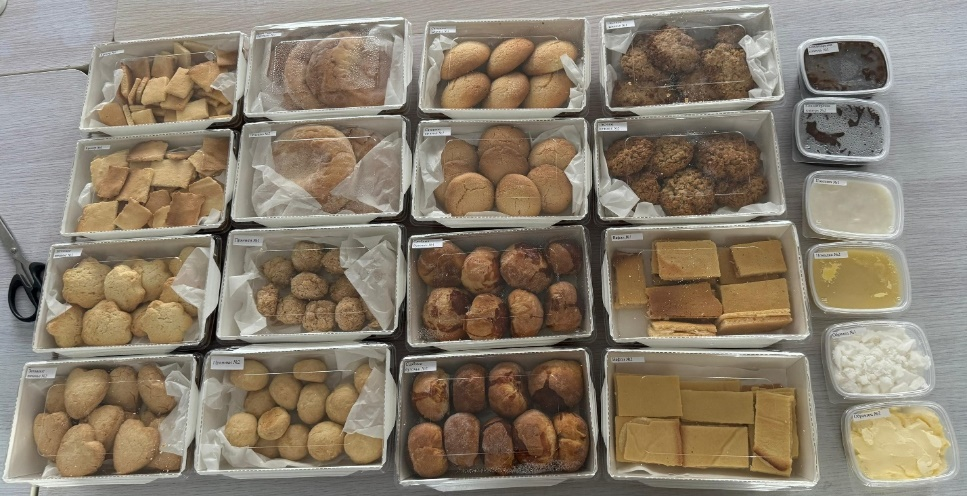
\includegraphics[width=0.8\textwidth]{media/pish/image11}
	\caption*{Fig.2 - Samples of bakery and confectionery products with the addition of vegetable fat and margarine}
\end{figure}

As a result, it was established that, in terms of organoleptic
indicators, products prepared with the addition of vegetable fat based
on hydrogenated oil are not inferior to products with the addition of
margarine. Also, the mass fraction of fat in bakery and confectionery
products was determined; the results of the studies are presented in
Table 1.

\tcap{Table 1 Mass fractions of fat in bakery and confectionery products}
\begin{longtblr}[
  label = none,
  entry = none,
]{
  width = \linewidth,
  colspec = {Q[44]Q[265]Q[296]Q[331]},
  cells = {c},
  hlines,
  vlines,
}
№  & Product name        & Mass fraction of fat, \% & ND on research methods \\
1  & Sugar cookies       & 10,6                     & GOST 31902-2012        \\
2  & Oatmeal cookies     & 11,2                     & GOST 31902-2012        \\
3  & Crackers            & 10,4                     & GOST 31902-2012        \\
4  & Gingerbread         & 10,7                     & GOST 31902-2012        \\
5  & Prolong cookies     & 10,3                     & GOST 31902-2012        \\
6  & Waffles             & 10,5                     & GOST 31902-2012        \\
7  & Flatbreads          & 9,4                      & GOST 5668-2022         \\
8  & Buns                & 3,5                      & GOST 5668-2022         \\
9  & Fudge               & 9,7                      & GOST 31902-2012        \\
10 & Confectionery glaze & 11,1                     & ГОСТ 31902-2012        
\end{longtblr}

Analyzing Table 1, it can be established that the mass fraction of fat
in bakery and confectionery products varied from 3.5\% to 11.2\%. The
content of TFA in the original oil and fat products was determined, the
results of the studies are shown in Table 2.

\tcap{Table 2 - TFA content in the original fat and oil products}
\begin{longtblr}[
  label = none,
  entry = none,
]{
  width = \linewidth,
  colspec = {Q[40]Q[458]Q[260]Q[183]},
  cells = {c},
  hlines,
  vlines,
}
№ & Product name                            & Mass fraction of fat, \% & TFA content, \% \\
1 & Vegetable fat based on hydrogenated oil & 99,7                     & 10,0            \\
2 & Margarine                               & 55,0                     & 0,31            
\end{longtblr}

\begin{figure}[H]
	\centering
	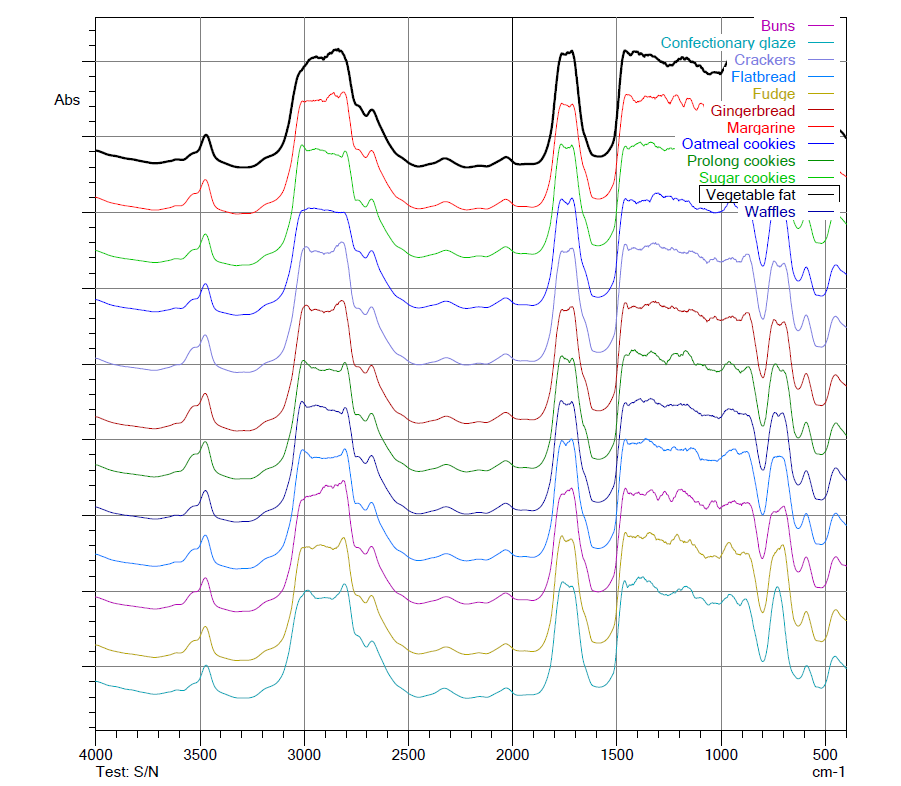
\includegraphics[width=0.6\textwidth]{media/pish/image12}
	\caption*{Fig.3 - IR spectra of the analyzed samples}
\end{figure}

\begin{multicols}{2}
The results of the studies showed that vegetable fat based on
hydrogenated oil exceeds the 2\% standard and is not suitable for direct
oral use. Margarine with a TFA content of 0.31\% complies with the
standards of TR CU 024/2011. However, it is important to note that
vegetable fat is presented as a fat product with a fat content of
99.7\%, and margarine is an emulsion product with a fat content of 55\%.
If margarine with a fat content of 55\% were prepared based on vegetable
fat, the TFA content would decrease to 5.5\%. Figure 3 shows the IR
spectra of the analyzed samples.

Next, the content of trans-isomers of fatty acids in bakery and
confectionery products with the addition of vegetable fat based on
hydrogenated oil was determined; the results are presented in Table 3.
\end{multicols}

\tcap{Table 3 - Content of trans-isomers of fatty acids in bakery and confectionery products}
\begin{longtblr}[
  label = none,
  entry = none,
]{
  width = \linewidth,
  colspec = {Q[40]Q[250]Q[168]Q[252]Q[287]},
  cells = {c},
  hlines,
  vlines,
}
№  & Product name        & Mass fraction of fat, \% & TFA content in extracted fat, \% & TFA content in finished products, \% \\
1  & Sugar cookies       & 10,6                     & 9,57                             & 1,01                                 \\
2  & Oatmeal cookies     & 11,2                     & 7,89                             & 0,88                                 \\
3  & Crackers            & 10,4                     & 9,28                             & 0,97                                 \\
4  & Gingerbread         & 10,7                     & 9,27                             & 0,99                                 \\
5  & Prolong cookies     & 10,3                     & 9,56                             & 0,98                                 \\
6  & Waffles             & 10,5                     & 9,76                             & 1,02                                 \\
7  & Flatbreads          & 9,4                      & 7,58                             & 0,71                                 \\
8  & Buns                & 3,5                      & 7,82                             & 0,27                                 \\
9  & Fudge               & 9,7                      & 8,63                             & 0,84                                 \\
10 & Confectionery glaze & 11,1                     & 10,48                            & 1,16                                 
\end{longtblr}

\begin{multicols}{2}
As can be seen from Table 3, the TFA content in all the listed bakery
and confectionery products does not exceed 2\%. Although vegetable fat
is not suitable as an independent oil and fat product for direct oral
use, it is quite suitable as an ingredient for other food products, such
as bakery and confectionery products.

According to the Order of the Chairman of the Sanitary and
Epidemiological Control Committee of the Ministry of Health of the
Republic of Kazakhstan dated 06/09/2023 No.69-NK, which approved the
methodological recommendations «Norms of physiological needs for energy
and nutrients for various groups of the population of the Republic of
Kazakhstan», the recommended fat content of the total energy value of
the daily diet for children under 6 months is 40-60\%, up to 2 years -
up to 35\%, 2-18 years - 25-35\%, adults - up to 30\%.

At the same time, the recommended content of saturated fats in the diet
is no more than 10\% of the total caloric content of the daily diet.
Consumption of trans-isomers of fatty acids should not exceed 1\% of the
caloric content of the daily diet. Also, according to the ASPR RK Bureau
of National Statistics, at the end of 2023, the energy value of food
products consumed by the population of the Republic of Kazakhstan was
3,129 kcal per day, of which the fat content is 32.6\%, that is, 1020
kcal per day. The maximum limit for the consumption of trans-isomers is
31.3 kcal per day. Then, the maximum level of trans-isomers in the daily
diet would be 3.1\%, which is higher than the established norm of TR CU
024/2011 TFA no more than 2\%. However, it is worth understanding that
this indicator includes not only oil and fat products, but all food
products.

{\bfseries Conclusion.} As noted earlier, the use of vegetable fat based on
hydrogenated oil does not exceed the standard content of TFA in bakery
and confectionery products, they can be considered safe for health.
Taking into account the daily consumption of these products, we consider
it necessary to allow domestic manufacturers of oil and fat products to
produce fats for special purposes for the bakery and confectionery
industry based on hydrogenated oils, bypassing the retail consumer
market, and directly make deliveries between business representatives.
It is necessary to work out the principles and stages of sales,
introduce tools for monitoring the safety of such sales so that
industrial margarines do not end up on consumer shelves. Against the
background of the economic situation in the country, associated with the
rise in the dollar and the growth of inflation for food products, this
decision could give a positive impetus to the entire food industry of
our country.

\emph{{\bfseries Financing} This research was funded by the Ministry of
Agriculture of the Republic of Kazakhstan (BR22886613).}
\end{multicols}

\begin{center}
{\bfseries References}
\end{center}

\begin{references}
1. Ferlay A., Bernard L., Meynadier A., Malpuech-Brugère C. Production
of trans and conjugated fatty acids in dairy ruminants and their
putative effects on human health: A review // Biochimie.
-2017.-Vol.141.- P.107-120. DOI 10.1016/j.biochi.2017.08.006

2. Islam M.A., Amin M.N., Siddiqui S.A., Hossain M.P., Sultana F., Kabir
M.R. Trans fatty acids and lipid profile: A serious risk factor to
cardiovascular disease, cancer and diabetes // Diabetes \& Metabolic
Syndrome. -2019.-Vol.13(2).- P.1643-1647. DOI 10.1016/j.dsx.2019.03.033

3. M. Mencin, H. Abramovič, E. Zlatić, L. Demšar, S. Piskernik,
M.Schreiner, K. Žmitek, A. Kušar, I. Pravst, R. Vidrih. Content of
trans-fatty acid isomers in bakery products on the Slovenian market //
LWT.- 2021.-Vol.143.- P.111095. DOI 10.1016/j.lwt.2021.111095

4. Stender S. In equal amounts, the major ruminant trans fatty acid is
as bad for LDL cholesterol as industrially produced trans fatty acids,
but the latter are easier to remove from foods // The American Journal
of Clinical Nutrition.-2015.-Vol.102(6).- P.1301-2.

DOI 10.3945/ajcn.115.123646

5. Wanders A.J., Alssema M., De Koning E.J. Fatty acid intake and its
dietary sources in relation with markers of type 2 diabetes risk: the
NEO study // European Journal of Clinical Nutrition. -- 2017. -Vol.
71(2.)-- P.245--251.
DOI:~\href{https://doi.org/10.1038/ejcn.2016.204}{10.1038/ejcn.2016.204}

6. Aronis K.N., Khan S.M., Mantzoros C.S. Effects of trans fatty acids
on glucose homeostasis: a meta-analysis of randomized,
placebo-controlled clinical trials // The American Journal of Clinical
Nutrition. -2012. -Vol.96(5).- P.1093--1099.
DOI~\href{https://doi.org/10.3945/ajcn.112.040576}{10.3945/ajcn.112.040576}

7. Mirmiran P., Hosseini S., Hosseinpour-Niazi S. Hydrogenated Vegetable
Oils and Trans Fatty Acids: Profile and Application to Diabetes //
Bioactive Food as Dietary Interventions for Diabetes. -2019.- P.19-32.
DOI 10.1016/B978-0-12-813822-9.00002-3

8. Costa N., Cruz R., Graça P., Breda J., Casal S. Trans fatty acids in
the Portuguese food market // Food Control.- 2016. -Vol.64. - P.
128-134. DOI 10.1016/j.foodcont.2015.12.010

9. Vučić V., Arsić A., Petrović S., Milanović S., Gurinović M., Glibetić
M. Trans fatty acid content in Serbian margarines: Urgent need for
legislative changes and consumer information //Food Chemistry. -2015.-
Vol.15(185).- P.437-440. DOI 10.1016/j.foodchem.2015.04.018

10. Micha R., Khatibzadeh S., Shi P. Global, regional, and national
consumption levels of dietary fats and oils in 1990 and 2010: a
systematic analysis including 266 country-specific nutrition surveys
//British Medical Journal. -2014.-Vol.348.-P. g2272. DOI
\href{https://doi.org/10.1136/bmj.g2272}{10.1136/bmj.g2272}

11. Ismail G., Abo El Naga R., El Sayed Zaki M., Jabbour J., \&
Al-Jawaldeh A. Analysis of Fat Content with Special Emphasis on Trans
Isomers in Frequently Consumed Food Products in Egypt: The First Steps
in the Trans Fatty Acid Elimination Roadmap // Nutrients.-2021.-Vol.
13(9). - P.3087. DOI 10.3390/nu13093087
\end{references}

\begin{authorinfo}
\emph{{\bfseries Information about the authors}}

Dalabayev A.- Master of Engineering and Technology, Senior Researcher of
the Astana branch of «Kazakh Research Institute of Processing and Food
Industry», Astana, Kazakhstan; e-mail: dalabaev\_askhat@mail.ru.

\emph{{\bfseries Информация об авторах}}

Далабаев А.Б. -- магистр техники и технологии, старший научный сотрудник
Астанинского филиала ТОО «Казахский научно-исследовательский институт
перерабатывающей и пищевой промышленности», Астана, Казахстан, е-mail:\\
dalabaev\_askhat@mail.ru
\end{authorinfo}
